\documentclass[aspectratio=169,11pt]{beamer}
% ==========================================================================
%  KSA lecture-slide theme  =  stock beamer "Boadilla"  +  KSA colour theme
%  brand colours sampled from the official KSA symbol mark:
%    Deep Prussian Blue  #2E3192   (지성 - intellect)
%    Golden Gray         #D6CBB1   (감성 - sensibility)
%  Engine: XeLaTeX.  Usage:
%    \documentclass[aspectratio=169,11pt]{beamer}
%    \input{../../theme/ksa-theme.tex}
%  Each deck lives in its own slides/kor/<deck>/ folder together with its
%  own images; ../../figs/ is kept only as a fallback for the shared cache.
% ==========================================================================

\usepackage{fontspec}
\usepackage{amsmath,amssymb}
\usepackage{graphicx}
\graphicspath{{figs/}{./}{../../../figs/}}
\usepackage{booktabs}
\usepackage{listings}
\usepackage{varwidth}

% ---- fonts (no ctex/xeCJK on this box -> fontspec drives CJK directly) -----
\defaultfontfeatures{Ligatures=TeX}
\setmainfont{Noto Sans CJK KR}
\setsansfont{Noto Sans CJK KR}
\setmonofont{Noto Sans Mono CJK KR}[Scale=0.92]

% ---- base theme: stock Boadilla ------------------------------------------
\usetheme{Boadilla}
\usefonttheme{professionalfonts}
\setbeamertemplate{navigation symbols}{}

% ---- KSA colour theme (recolour the stock theme) --------------------------
\definecolor{ksablue}{HTML}{2E3192}
\definecolor{ksabluedk}{HTML}{20226A}
\definecolor{ksagold}{HTML}{D6CBB1}
\definecolor{ksagolddk}{HTML}{A9976B}
\definecolor{ksared}{HTML}{C0392B}
\definecolor{ksagray}{HTML}{5B5B5B}

\setbeamercolor{structure}{fg=ksablue}
\setbeamercolor{alerted text}{fg=ksared}

\setbeamercolor{palette primary}{fg=white,           bg=ksablue}
\setbeamercolor{palette secondary}{fg=white,         bg=ksablue!85!black}
\setbeamercolor{palette tertiary}{fg=white,          bg=ksabluedk}
\setbeamercolor{titlelike}{fg=ksablue}
\setbeamercolor{frametitle}{fg=ksablue,bg=}
\setbeamercolor{title}{fg=ksablue}
\setbeamercolor{author}{fg=ksagray}
\setbeamercolor{institute}{fg=ksagray}
\setbeamercolor{block title}{fg=white,bg=ksablue}
\setbeamercolor{block body}{fg=black!85,bg=ksablue!6}
\setbeamercolor{item}{fg=ksablue}
\setbeamercolor{section in toc}{fg=black!85}

\setbeamerfont{frametitle}{series=\bfseries}
\setbeamerfont{title}{series=\bfseries}

% ---- footline:  KSA mark | "Made by ..." | n / N   (matches reference) ----
\newcommand{\ksacredit}{}
\setbeamertemplate{footline}{%
  \hbox{%
    \begin{beamercolorbox}[wd=.18\paperwidth,ht=2.6ex,dp=1.5ex,leftskip=1.1em]{}%
      \raisebox{-0.35ex}{\includegraphics[height=2.0ex]{ksa-logo.png}}%
    \end{beamercolorbox}%
    \begin{beamercolorbox}[wd=.64\paperwidth,ht=2.6ex,dp=1.5ex,center]{}%
      {\scriptsize\color{ksagray}\ksacredit}%
    \end{beamercolorbox}%
    \begin{beamercolorbox}[wd=.18\paperwidth,ht=2.6ex,dp=1.5ex,rightskip=1.1em]{}%
      \hfill{\scriptsize\color{ksablue}\insertframenumber\,/\,\inserttotalframenumber}%
    \end{beamercolorbox}%
  }%
  \vskip2pt
}

% ---- section divider: stock \sectionpage, KSA-coloured -------------------
\setbeamertemplate{section page}{%
  \begingroup\centering
    {\color{ksagolddk}\rule{0.16\paperwidth}{1pt}}\par\vskip1.0em
    {\usebeamerfont{title}\color{ksablue}\insertsectionhead\par}\vskip1.0em
    {\color{ksagolddk}\rule{0.16\paperwidth}{1pt}}\par
  \endgroup
}
\AtBeginSection[]{\begin{frame}[plain,noframenumbering]\vfill\sectionpage\vfill\end{frame}}

% ---- code listings ------------------------------------------------------------
\lstdefinestyle{ksa}{%
  basicstyle=\ttfamily\scriptsize,
  keywordstyle=\color{ksablue}\bfseries,
  commentstyle=\color{ksagray}\itshape,
  stringstyle=\color{ksagolddk},
  numberstyle=\tiny\color{ksagray},
  backgroundcolor=\color{ksablue!6},
  frame=leftline, framerule=1.4pt, rulecolor=\color{ksablue},
  xleftmargin=1em, aboveskip=0.8em, belowskip=0.4em,
  showstringspaces=false, breaklines=true, language=Python,
}
\lstset{style=ksa}

% ---- handy macros -----------------------------------------------------------
\newcommand{\kb}[1]{\textbf{\color{ksablue}#1}}   % blue keyword
\newcommand{\kq}[1]{\textbf{\color{ksared}#1}}    % red key-question

\setbeamerfont{title}{series=\bfseries,size=\fontsize{24}{30}\selectfont}
\setbeamerfont{subtitle}{series=\bfseries,size=\fontsize{14}{18}\selectfont}
\setbeamerfont{author}{size=\normalsize}
\setbeamerfont{institute}{size=\small}
\graphicspath{{figs/}{../../../../assets/}}
\makeatletter
\newcommand{\markpage}[1]{\protected@write\@auxout{}{\string\newlabel{#1}{{\the\c@framenumber}{}}}\hypertarget{#1}{}}
\newcommand{\pref}[1]{\hyperlink{#1}{\textcolor{ksagolddk}{(p.\ref{#1})}}}
\makeatother

\renewcommand{\ksacredit}{Machine Learning 1 \,\textperiodcentered\, GAN}
\title{GAN 생성적 적대 신경망 (Generative Adversarial Network)}
\subtitle{위조범과 경찰이 겨루며 함께 는다}
\author{Machine Learning 1}
\institute{한국과학영재학교 (KSA)}
\date{}
\begin{document}
\begin{frame}[plain,noframenumbering]\titlepage\end{frame}


% --- 오늘의 질문
\begin{frame}{오늘의 질문: ``진짜 같다'' 를 어떻게 손실로 만들까?}
\vfill
\centering
{\large VAE: 원래 그림과 \textbf{칸마다} 비교 (복원 오차) $\to$ 평균 내다 보니 흐리다}\vskip0.6em
{\large 진짜 같음은 칸마다 비교로 못 잰다: 같은 7 도 쓰는 법이 수천 가지}\vskip0.6em
{\large 아이디어: 진짜와 가짜를 가려내는 \kb{신경망을 하나 더} 두고, 그걸 속이게 하자}\\[0.4em]
{\small Goodfellow 외 (2014) ``Generative Adversarial Nets'' \quad 요슈아 벤지오 교수 팀}
\vfill
\note{지난 덱의 VAE는 되살린 그림을 원래 그림과 칸마다 비교했습니다. 여러 가능성을 평균 내다 보니 그림이 흐렸죠. 그런데 진짜 같다는 건 칸마다 비교로 잴 수 없습니다. 같은 숫자 7도 쓰는 법이 수천 가지니까요. 2014년 이언 굿펠로와 요슈아 벤지오 교수 팀은 이렇게 생각했습니다. 진짜와 가짜를 가려내는 신경망을 하나 더 두고, 그 신경망을 속이도록 학습시키자. 이게 GAN, 생성적 적대 신경망입니다.}
\end{frame}

% --- 구조
\begin{frame}{위조범과 경찰}
\markpage{scheme}
\vfill
\centering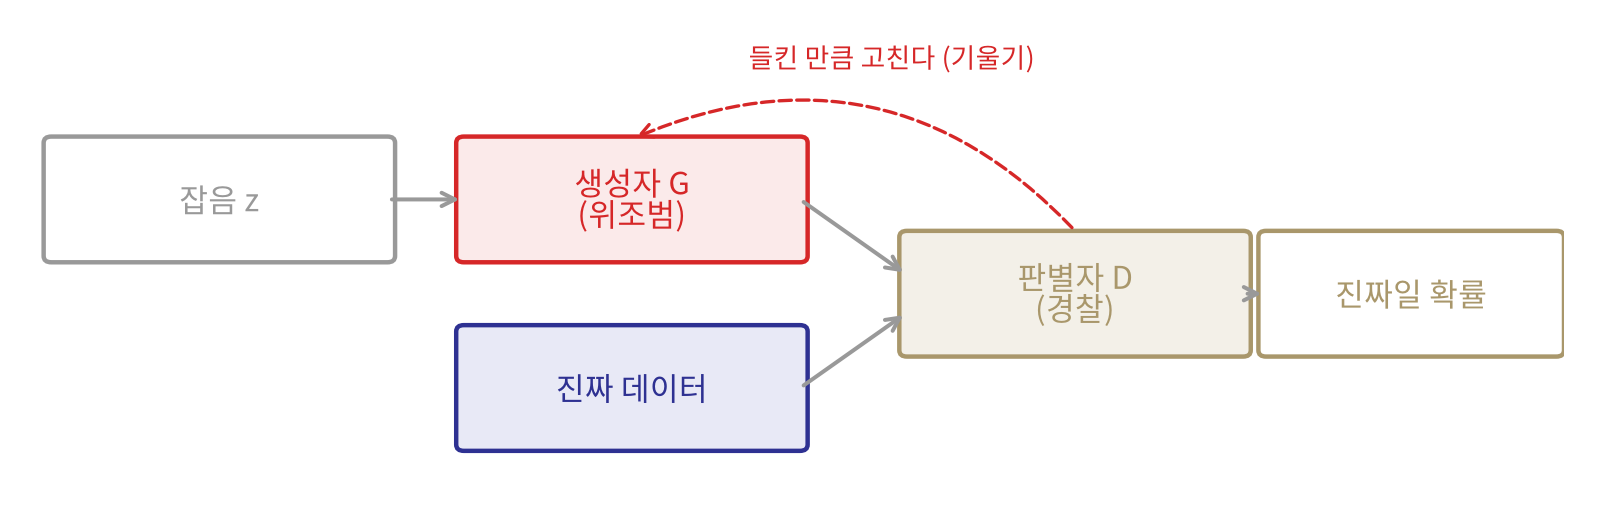
\includegraphics[width=0.84\linewidth]{gan_scheme.png}\par\vskip0.2em
\renewcommand{\arraystretch}{1.4}
{\large\begin{tabular}{ll}
\textcolor{ksared}{생성자 $G$} & 잡음 $\mathbf{z}$ $\to$ 가짜 \quad 목표: $D$ 가 가짜를 진짜라고 믿게\\
\textcolor{ksagolddk}{판별자 $D$} & 그림 $\to$ 진짜일 확률 \quad 목표: 진짜는 1, 가짜는 0
\end{tabular}}
\vfill
\note{GAN에는 신경망이 둘 있습니다. 생성자 G는 위조범입니다. 잡음 z를 받아 가짜 그림을 만들고, 판별자가 진짜라고 믿게 하는 게 목표입니다. 판별자 D는 경찰입니다. 그림을 받아 진짜일 확률을 내고, 진짜에는 1, 가짜에는 0을 주는 게 목표입니다. 경찰에게 들키면, 위조범은 들킨 만큼, 즉 판별자를 통해 흘러온 기울기만큼 가짜를 고칩니다. 둘이 겨루며 함께 늘어 갑니다.}
\end{frame}

% --- 식
\begin{frame}{식으로: 두 사람의 게임}
\markpage{formula}
\vfill
\centering
{\LARGE\[ \min_G \max_D \; \mathbb{E}_{\mathbf{x} \sim \text{진짜}} \big[\log D(\mathbf{x})\big] + \mathbb{E}_{\mathbf{z}} \big[\log\big(1 - D(G(\mathbf{z}))\big)\big] \]}\vskip0.4em
\renewcommand{\arraystretch}{1.5}
{\large\begin{tabular}{ll}
$D$ 한 걸음 & 진짜는 1, 가짜는 0 으로 맞히는 이진 교차 엔트로피를 줄인다\\
$G$ 한 걸음 & 가짜에 대해 ``진짜 (1)'' 를 정답으로 한 교차 엔트로피를 줄인다 (실전 꼴)\\
번갈아 & $D$ 한 걸음, $G$ 한 걸음, $\cdots$
\end{tabular}}\\[0.4em]
{\large 이상적인 끝: 가짜가 진짜와 같아지면 $D$ 는 무엇이든 \kb{1/2}}
\vfill
\note{식으로 쓰면 두 사람의 게임입니다. 판별자는 진짜에 로그 D, 가짜에 로그 1 빼기 D를 크게 하려 하고, 생성자는 이걸 작게 하려 합니다. 실제 학습은 번갈아 합니다. 판별자 한 걸음은 진짜는 1, 가짜는 0으로 맞히는 이진 교차 엔트로피를 줄이고, 생성자 한 걸음은 가짜에 진짜, 1을 정답으로 준 교차 엔트로피를 줄입니다. 논문이 권한 실전 꼴입니다. 가짜가 진짜와 똑같아지면 판별자는 무엇을 봐도 2분의 1이라고 할 수밖에 없습니다. 원 논문이 증명한 이상적인 끝입니다.}
\end{frame}

% --- 손 계산
\begin{frame}{손으로 한 번: 판별자의 점수}
\vfill
\centering
{\large 판별자가 진짜 그림에 0.9, 가짜 그림에 0.2 를 줬다}\vskip0.6em
\renewcommand{\arraystretch}{1.6}
{\Large\begin{tabular}{ll}
$D$ 의 손실 & $-\ln 0.9 - \ln(1 - 0.2) = 0.105 + 0.223 = \kb{0.33}$\\
$G$ 의 손실 & $-\ln 0.2 = \kq{1.61}$ \quad (들켰다: 크다)
\end{tabular}}\vskip0.6em
{\large 끝에 $D$ 가 모두 0.5 를 주면: \quad $D$ 손실 $2\ln 2 = 1.39$, \quad $G$ 손실 $\ln 2 = 0.69$}
\vfill
\note{판별자가 진짜 그림에 0.9, 가짜 그림에 0.2를 줬다고 합시다. 판별자의 손실은 마이너스 로그 0.9 더하기 마이너스 로그 0.8, 0.105 더하기 0.223, 0.33으로 작습니다. 잘 가려내고 있으니까요. 생성자의 손실은 마이너스 로그 0.2, 1.61로 큽니다. 들켰으니까요. 학습이 끝나 판별자가 모두 0.5를 주면 판별자 손실은 2 곱하기 로그 2, 1.39, 생성자 손실은 로그 2, 0.69가 됩니다.}
\end{frame}

% --- 실험 고리
\begin{frame}{실험 1: 고리 모양 데이터}
\markpage{ring}
\vfill
\centering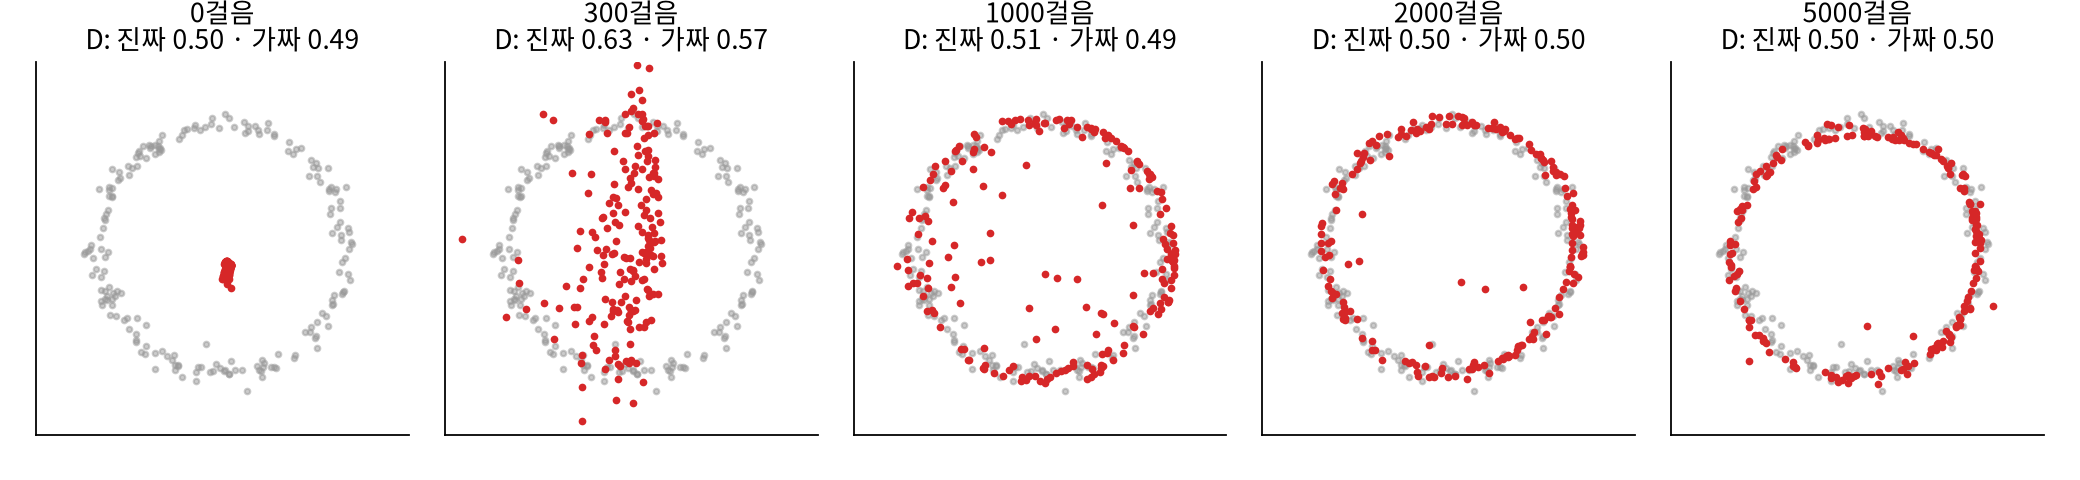
\includegraphics[width=0.96\linewidth]{gan_ring.png}\par\vskip0.3em
{\large 회색 = 진짜 (반지름 2 고리), 빨강 = 생성자의 가짜 \quad 같은 잡음 200개로 단계별}\\[0.2em]
{\large 300걸음: 판별자가 진짜에 0.63 \quad 5,000걸음: 진짜도 가짜도 \kb{0.50}}
\vfill
\note{2차원 장난감으로 직접 해 봤습니다. 회색이 진짜 데이터, 반지름 2인 고리 위의 점들이고, 빨간 점이 생성자가 만든 가짜입니다. 처음에는 가운데 뭉쳐 있다가, 300걸음에는 판별자가 진짜에 0.63을 줄 만큼 가려내고, 1000, 2000걸음을 지나며 가짜 점이 고리를 따라 퍼집니다. 5000걸음에는 판별자가 진짜에도 가짜에도 0.50을 줍니다. 더는 못 가려낸다는 뜻입니다.}
\end{frame}

% --- 모드 붕괴
\begin{frame}{실험 2: 불안정한 학습 · 모드 붕괴}
\markpage{eight}
\vfill
\begin{columns}[c]
\column{0.55\linewidth}\centering
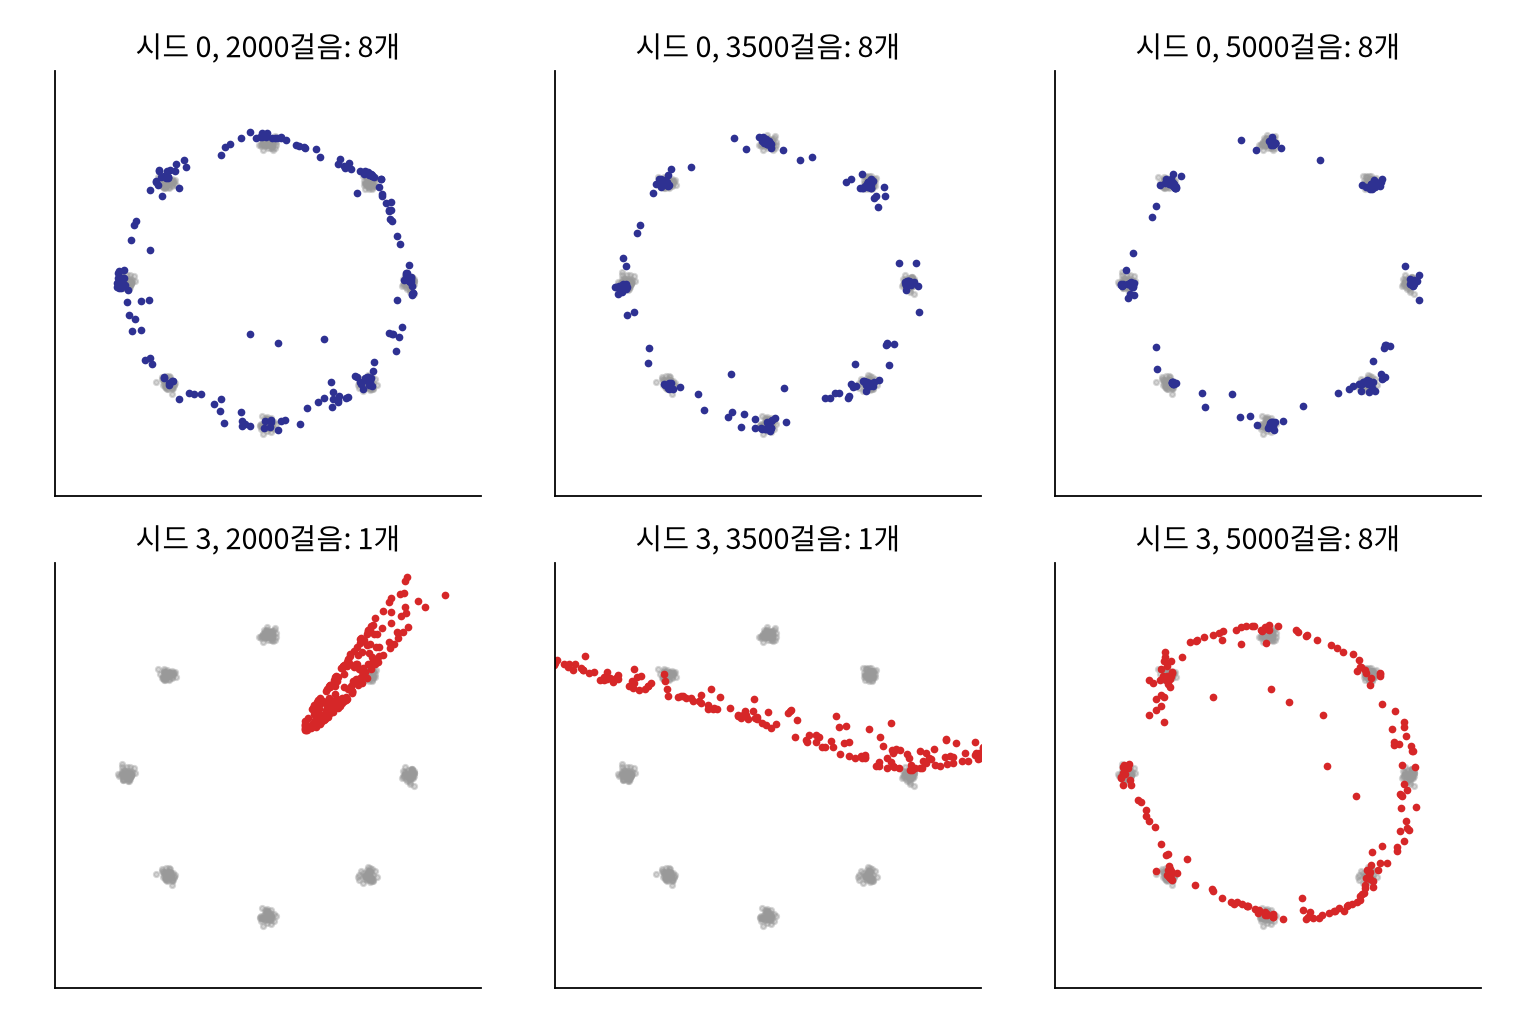
\includegraphics[width=\linewidth]{gan_eight.png}
\column{0.43\linewidth}
{\large 봉우리 8개, 같은 설정 · 시드만 다르게}\\[0.6em]
{\large 시드 5개 중 4개: 1,500걸음에 \kb{8개} 모두}\\[0.4em]
{\large 시드 3: 4,500걸음까지 \kq{0 $\sim$ 1개} 를 맴돌다 5,000걸음에야 8개}\\[0.8em]
{\small 생성자가 판별자의 약한 곳 한 군데만 노리면 한 모양만 만든다 (모드 붕괴)}
\end{columns}
\vfill
\note{두 번째 실험은 원 위의 봉우리 8개입니다. 같은 설정에 시드만 다르게 다섯 번 학습했습니다. 다섯 번 중 네 번은 1500걸음에 8개 봉우리를 모두 덮었습니다. 그런데 시드 3은 4500걸음까지 봉우리를 0개에서 1개만 덮으며 엉뚱한 곳을 맴돌다 5000걸음에야 8개를 덮었습니다. 판별자와 생성자가 서로 쫓고 쫓기다 보니 학습이 불안정합니다. 생성자가 판별자의 약한 곳 한 군데만 노리면 한 모양만 만들게 되는데, 이걸 모드 붕괴라고 합니다.}
\end{frame}

% --- 숫자
\begin{frame}{실험 3: 손글씨 숫자}
\markpage{digits}
\vfill
\centering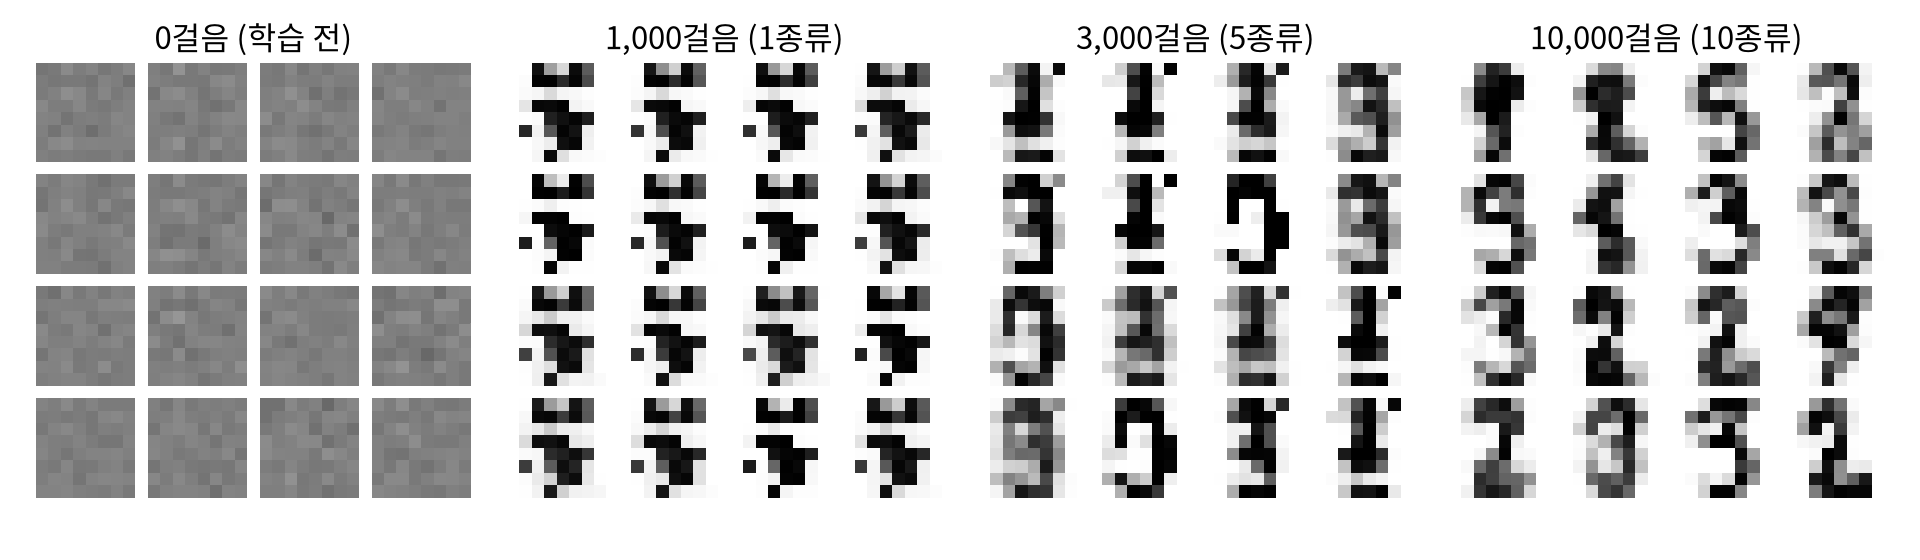
\includegraphics[width=0.9\linewidth]{gan_digits.png}\par\vskip0.2em
{\large 1,000걸음: 2,000장 \kq{모두 ``5''} (모드 붕괴) \quad 3,000걸음: 5종류 \quad 10,000걸음: \kb{10종류}}\\[0.2em]
{\small 숫자 판정 = 원본으로 학습한 로지스틱 회귀 \quad 확신 (확률 0.9 이상) 36\%, 원본 사진은 77\%}
\vfill
\note{세 번째는 손글씨 숫자입니다. 1000걸음에는 2000장을 뽑았는데 모두 같은 5 모양입니다. 모드 붕괴가 그대로 보입니다. 3000걸음에는 다섯 종류, 10000걸음에는 열 종류가 모두 나옵니다. 분류기가 0.9 이상 확신한 비율은 36퍼센트로, 원본 사진 77퍼센트보다는 낮습니다. 8 곱하기 8의 작은 그림과 작은 신경망이라 아직 거칠지만, 판별자 하나만으로 숫자 모양을 배워 낸 겁니다.}
\end{frame}

% --- 역사
\begin{frame}{GAN 이 연 길}
\vfill
\centering
\renewcommand{\arraystretch}{1.5}
{\large\begin{tabular}{ll}
2014 & GAN (Goodfellow 외): 흐릿한 작은 그림\\
2015 & DCGAN: 합성곱으로, 안정적인 학습 요령\\
2017 & CycleGAN: 말 $\leftrightarrow$ 얼룩말, 사진 $\leftrightarrow$ 그림 (짝 없는 변환)\\
2018 $\sim$ 2019 & StyleGAN: 진짜 같은 1024 × 1024 얼굴 (딥페이크 논란도)\\
2020 $\sim$ & 확산 모델이 주도: 학습이 안정적이고 다양하다 (다음 덱)
\end{tabular}}\vskip0.6em
{\large 장점: 한 번에 빠르게 생성, 선명 \quad 약점: 불안정한 학습, 모드 붕괴}
\vfill
\note{GAN은 2014년 흐릿한 작은 그림에서 시작해, 2015년 DCGAN이 합성곱 신경망과 안정적인 학습 요령을 정리했고, 2017년 CycleGAN은 말 사진을 얼룩말로, 사진을 그림으로 짝 없이 바꿨습니다. 2018년 StyleGAN은 실제와 구분하기 힘든 1024 곱하기 1024 얼굴을 만들었는데, 딥페이크 논란도 함께 생겼습니다. 2020년 이후에는 학습이 안정적이고 다양한 그림을 만드는 확산 모델이 주도권을 가져갔습니다. GAN의 장점은 한 번에 빠르게 선명한 그림을 만드는 것, 약점은 불안정한 학습과 모드 붕괴입니다.}
\end{frame}

% --- 문제풀이
\begin{frame}{문제풀이}
\vfill
\begin{enumerate}
\item 판별자가 진짜에 0.6, 가짜에 0.6 을 줬다. $D$ 의 손실과 $G$ 의 손실은? ($\ln 0.6 \approx -0.51$, $\ln 0.4 \approx -0.92$)\vskip0.8em
\item 판별자가 너무 잘해서 가짜에 항상 0.0001 을 주면, $\log(1 - D(G(z)))$ 를 줄이는 생성자의 기울기는 어떻게 될까?\vskip0.8em
\item 모드 붕괴가 생기면 2,000장을 뽑았을 때 무엇이 보일까? 어떻게 알아챌 수 있을까?\vskip0.8em
\item VAE 와 GAN 을 ``흐림 · 다양함 · 학습 안정성'' 으로 비교해 보라.
\end{enumerate}
\vfill
\note{1번 답. 판별자 손실은 마이너스 로그 0.6 더하기 마이너스 로그 0.4, 0.51 더하기 0.92, 1.43이고, 생성자 손실은 마이너스 로그 0.6, 0.51입니다. 2번 답. 1 빼기 D가 거의 1이라 로그가 거의 평평해 기울기가 거의 0이 됩니다. 그래서 실전에서는 마이너스 로그 D를 줄이는 꼴을 씁니다. 3번 답. 거의 같은 그림만 반복됩니다. 실험처럼 분류기로 종류를 세거나, 뽑은 그림끼리 얼마나 다른지 재면 알 수 있습니다. 4번 답. VAE는 흐리지만 다양하고 학습이 안정적이고, GAN은 선명하지만 모드 붕괴로 다양성이 줄 수 있고 학습이 불안정합니다.}
\end{frame}

% --- 실습
\begin{frame}{실습}
\vfill
\centering\begin{tabular}{rl}
\large 1 & 판별자 · 생성자 손실 손 계산 (0.33, 1.61)\\[0.5em]
\large 2 & 2차원 GAN: 고리 · 봉우리 8개, 덮은 봉우리 수 세기\\[0.5em]
\large 3 & 손글씨 숫자 GAN, 단계별 그림 · 종류 수
\end{tabular}\vskip1em
\href{https://colab.research.google.com/github/SuminHan/book-ml/blob/main/slides/v2/ml1/week15/gan/lab/gan.ipynb}{\textcolor{ksagolddk}{▶ Colab에서 실습 노트북 열기}}
\vfill
\note{실습은 세 부분입니다. 첫째, 판별자와 생성자의 손실을 손으로 계산합니다. 둘째, 2차원 GAN으로 고리와 봉우리 8개를 학습하며 덮은 봉우리 수를 셉니다. 셋째, 손글씨 숫자 GAN을 학습해 단계별 그림과 종류 수를 봅니다.}
\end{frame}

% --- 정리
\begin{frame}{정리}
\vfill
\centering\large\begin{tabular}{l}
\textbf{GAN}: 생성자 (위조범) vs 판별자 (경찰), 번갈아 학습 (2014)\\[0.5em]
판별자: 진짜 1 · 가짜 0 \quad 생성자: 가짜를 ``진짜'' 로 믿게 \quad 끝: $D = 1/2$\\[0.5em]
고리: 5,000걸음에 진짜 · 가짜 모두 0.50 \quad 봉우리 8개: 시드 하나는 오래 1개\\[0.5em]
숫자: 1,000걸음 전부 ``5'' (모드 붕괴) $\to$ 10,000걸음 10종류 \quad 다음: 확산 모델
\end{tabular}
\vfill
\note{정리합니다. GAN은 위조범인 생성자와 경찰인 판별자를 번갈아 학습시킵니다. 판별자는 진짜에 1, 가짜에 0을 주려 하고, 생성자는 가짜를 진짜로 믿게 하려 하며, 이상적인 끝에서 판별자는 무엇이든 2분의 1을 줍니다. 고리 실험에서 5000걸음에 진짜와 가짜 모두 0.50을 받았고, 봉우리 8개 실험에서는 한 시드가 오랫동안 봉우리 하나에 머물렀습니다. 숫자 실험에서는 1000걸음에 모두 5를 만드는 모드 붕괴가 보였다가, 10000걸음에 열 종류가 나왔습니다. 다음 덱에서는 확산 모델을 배웁니다.}
\end{frame}
\end{document}
